\documentclass[12pt]{article}
\usepackage[letterpaper,top=2.54cm,bottom=2.54cm,left=2.54cm,right=2.54cm,marginparwidth=1.75cm]{geometry}
%% Language and font encodings
\usepackage[english]{babel}
\usepackage[utf8x]{inputenc}
\usepackage[T1]{fontenc}
\usepackage{graphicx}
\usepackage{subcaption}
\usepackage{mwe}
\usepackage{float}
\usepackage{amsmath}
\usepackage{multicol}
\usepackage[colorinlistoftodos]{todonotes}
\usepackage[colorlinks=true, allcolors=blue]{hyperref}
\usepackage{listings}
\usepackage{mathptmx}
\usepackage{color}
\usepackage{amsmath}
\usepackage{amssymb}
\usepackage{epstopdf}
\usepackage{inputenc}
\usepackage{geometry}
\usepackage{color}
\usepackage[nottoc]{tocbibind}
\usepackage{natbib}
\usepackage{courier}
\usepackage{algorithm}
\usepackage[noend]{algpseudocode}
\usepackage{qtree}
\usepackage{forest}
\usepackage{datetime}

\makeatletter
\def\BState{\State\hskip-\ALG@thistlm}
\makeatother

%% Matlab
\definecolor{mygreen}{RGB}{28,172,0} % color values Red, Green, Blue
\definecolor{mylilas}{RGB}{170,55,241}

\lstset{language=C++,%
    basicstyle=\scriptsize\ttfamily,
    breaklines=true,%
    morekeywords={matlab2tikz},
    keywordstyle=\color{blue},%
    morekeywords=[2]{1}, keywordstyle=[2]{\color{black}},
    identifierstyle=\color{black},%
    stringstyle=\color{mylilas},
    commentstyle=\color{mygreen},%
    showstringspaces=false,%without this there will be a symbol in the places where there is a space
    numbers=left,%
    numberstyle={\tiny \color{black}},% size of the numbers
    numbersep=9pt, % this defines how far the numbers are from the text
    emph=[1]{for,end,break},emphstyle=[1]\color{red}, %some words to emphasise
    emph=[2]{word1,word2}, emphstyle=[2]{style},    
}


\begin{document}
\begin{titlepage}
	\centering
	{\scshape\LARGE Columbia University \par}
	\vspace{1cm}
	{\scshape MECE 4510 Evolutionary Computation and Design Automation\par}
	\vspace{1.5cm}
	{\huge\bfseries Assignment\ 3\ -\ Phase B\par}
	\vspace{2cm}
	{\Large\itshape Hanwen Zhao\par}
	{UNI: hz2547\par}
	\vfill
	supervised by\par
	Dr.~Hod \textsc{Lipson}
	\vfill
	Grace Hours Used: 129\\
	Grace Hours Accumulated: 70\\
	Grace Hours Remaining: 37 \\
	\vspace{2cm}
% Bottom of the page
	{\large \today \ \currenttime \par}
\end{titlepage}

\newpage
\section{Result Summary}
\begin{figure}[H]
	\centering
	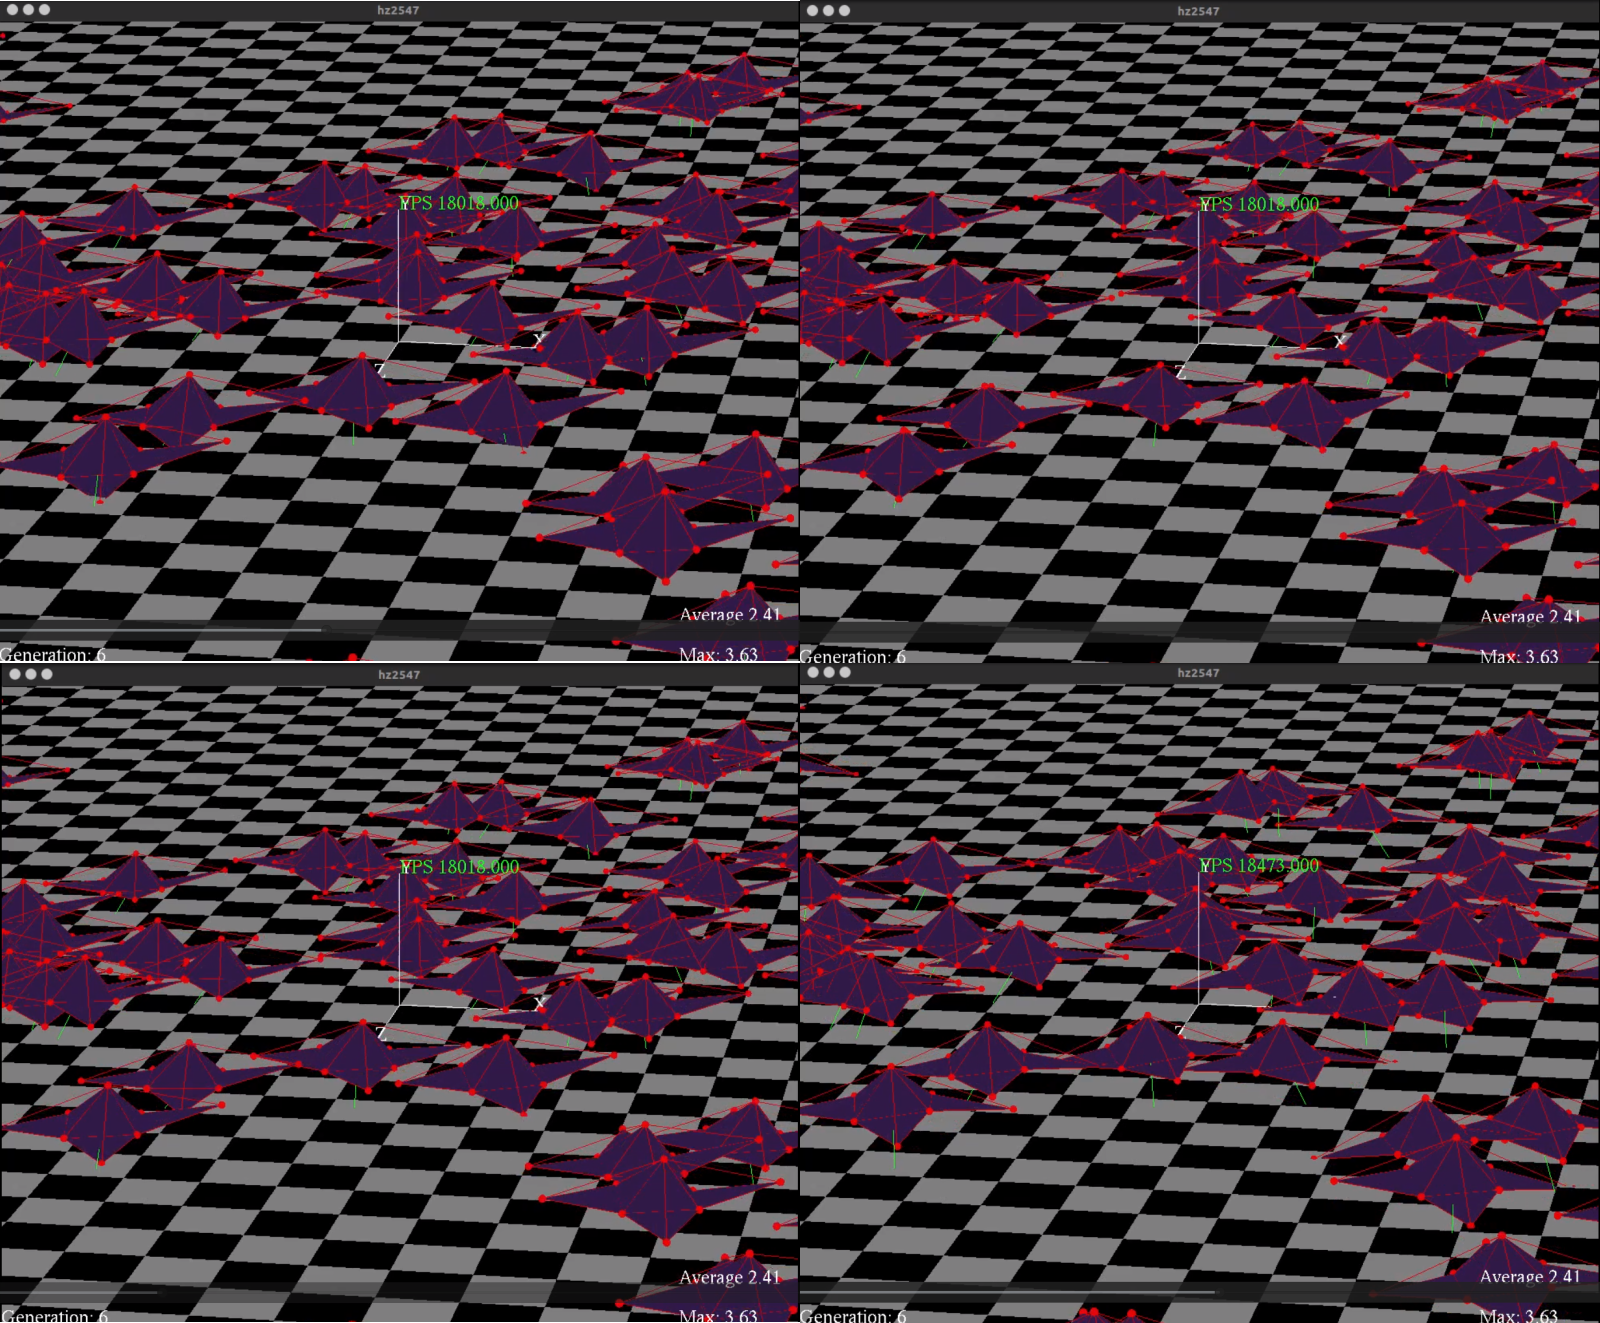
\includegraphics[width=0.7\textwidth]{combine_images}
	\caption[]%
	{{\small Group of Fastest Robots Moving 0.0163m/s}}    
\end{figure}
url: \url{https://goo.gl/2Gmhao}

\begin{figure}[H]
	\centering
	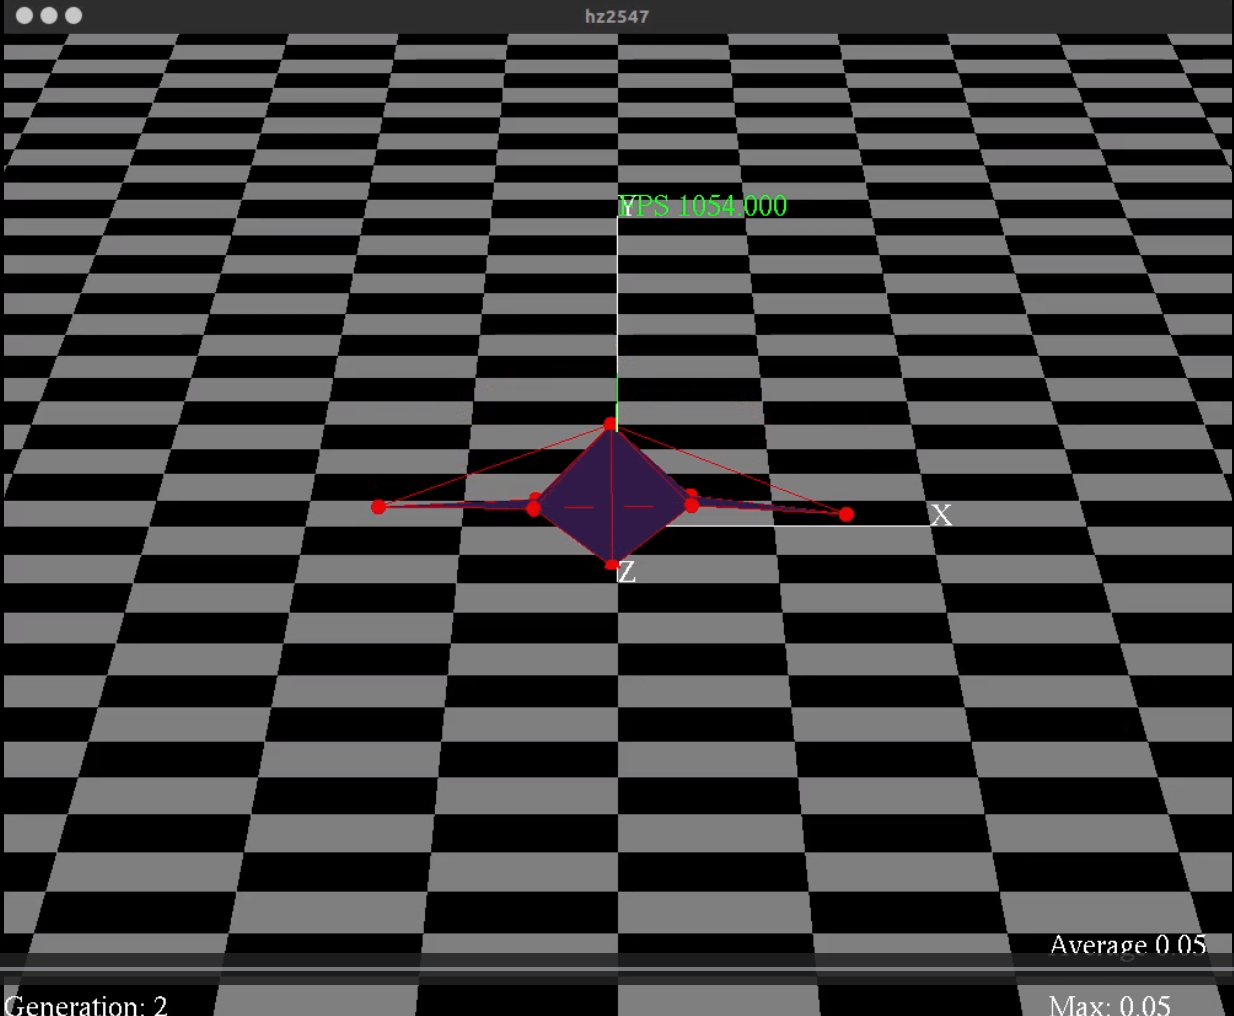
\includegraphics[width=0.5\textwidth]{bouncing}
	\caption[]%
	{{\small Bouncing Test}}    
\end{figure}
\noindent
url: \url{https://goo.gl/fsHNQN}


\newpage
\section{Methods}
\subsection{Description of Design}
At the second phase of the project, we are going to evolve a controller for a robot with fixed morphology. First, I created a robot based on a tetrahedron. The robot is shown in the following picture. The tetrahedron base contains 5 masses and 10 springs with high spring constant. Then, I added four legs to the tetrahedron with four softer springs to control them. Hope these four legs could help the robot to move faster.
From the previous phase of assignment 3, I built a simulation based on C++ and OpenGL. In this part of the project, the main goal is to code the classes for building the robot and implement evolutionary algorithm.

\subsubsection{EA Representation}
There are four legs in each robot, and each leg is controlled by one soft spring. The rest length of each soft spring is controlled by the following equation:
\begin{center}
	\begin{equation}
		L = L_0 + A*sin(B*t+C)
	\end{equation}
\end{center}
Therefore, there are 3 parameters for each leg, 12 parameters for each robot. In this assignment, I am using direct encoding to see how it works, which means each robot is evolved by a 12 numbers gene.
\subsubsection{Design Parameters}
The following are the parameter I used for this phase of the assignment:\\
Simulation Parameters:
\begin{itemize}
	\setlength\itemsep{0em}
	\item simulation time = 200 s (frame time)
	\item time step = 0.001 s
	\item ground restoration constant  = 10000 N/m
	\item dampening constant = 0.99
	\item ground friction coefficient = 0.7
	\item gravity = 9.81 N/kg
\end{itemize}
Robot Parameters:
\begin{itemize}
\setlength\itemsep{0em}
\item mass = 0.5 kg
\item length of tetrahedron = 1 m
\item soft spring constant = 1000 N/m
\item hard spring constant = 5000 N/m
\item Gene A range =\  -1 - 1
\item Gene B range =\  -$\pi$/2 - $\pi$/2
\item Gene C range =\  -2*$\pi$ - 2*$\pi$
\end{itemize}
Evolutionary Parameters:
\begin{itemize}
	\setlength\itemsep{0em}
	\item population size = 128
	\item mutation probability = 0.9
	\item number of points for crossover = 2
\end{itemize}


\subsection{Analysis}
Simulation:\\
Overall working with C++ and OpenGL gets more smoothly. The overall speed of simulation is satisfying. However, there is major issue with simulation is that the simulation returns different distance for the robots with the same gene. This might due to the calculation error due to the quick length change in the robot arm causing big forces. When the time step is not small enough to update the following acceleration and velocity change, this error could happen. This also reflect to the learning curve plot where the best fitness in each generation could go down.\\
\\
Robot:\\
The tetrahedron was a good way to start, however with simple spring-mass simulation, it is hard to build a "hard" robot. The final result proofed that the robot eventually wriggling on the ground to move instead of using arms to "walk".\\
\\
Evolutionary Algorithm:\\
In this part of the project, I am only using two point crossover and simple mutation to evolve the gene for each generation. This actually shows that my EA has poor linkage and diversity. This mainly due to that the structure I designed for simulation is hard to calculate the fitness for one single robot so that deterministic crowding could be used to maintain diversity.\\
Number of springs evaluations: ~810000/s




\newpage
\section{Performance}
\subsection{Performance Plots}
\begin{figure}[H]
	\centering
	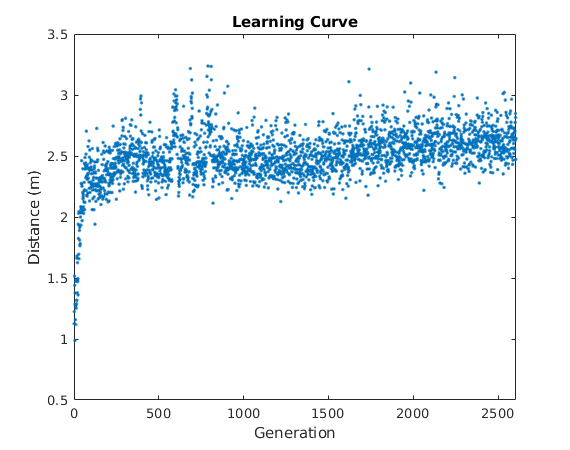
\includegraphics[width=0.7\textwidth]{learning_curve}
	\caption[]%
	{{\small Learning Curve}}    
\end{figure}

\newpage
\section{Additional Tasks}
\subsection{Dot Chart}
\begin{figure}[H]
	\centering
	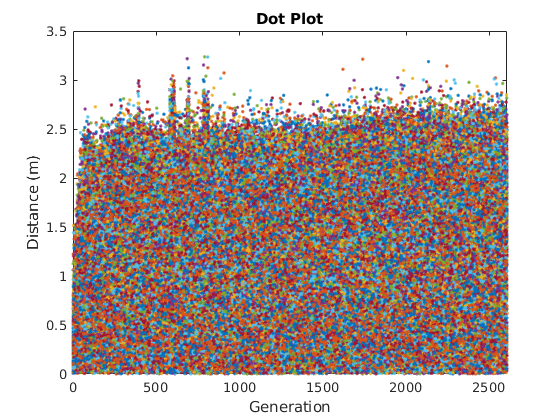
\includegraphics[width=0.6\textwidth]{dot_plot}
	\caption[]%
	{{\small Dot Chart}}    
\end{figure}


\subsection{Diversity Chart}
\begin{figure}[H]
	\centering
	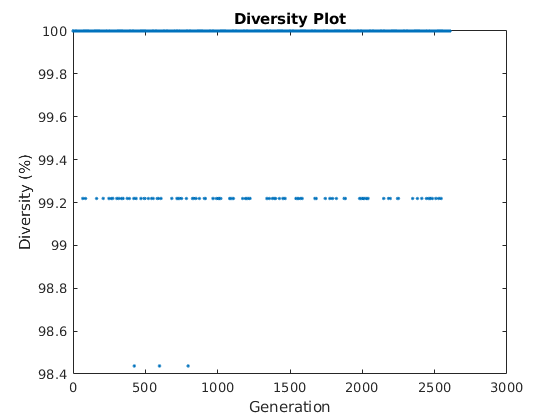
\includegraphics[width=0.6\textwidth]{diversity}
	\caption[]%
	{{\small Diversity Chart}}    
\end{figure}



\newpage
\section{Appendix}
\lstinputlisting{main.cpp}



\end{document}